\section{A neural proposal model}\label{sec:network}
This section describes one predictor that can rank candidate releases and supply bets. It is not needed for Theorem~\ref{M-thm:gate}, which holds for any predictable bet, and nothing here bears on the validity of the gate.

\subsection{SENTRY-R and its evidence streams}
SENTRY-R (scenario-enriched neural triage for release review) keeps three streams apart (Figure~\ref{fig:sentry}): scenarios suggested by a large language model (LLM) or by reviewers, which can enlarge the threat model but supply no outcomes; measured development attack counts, which train the predictor; and final audit outcomes, which alone can certify. A human reviewer must decide whether a proposed auxiliary source is lawful, accessible and distinct from an existing attack; the software checks a fixed feature schema and records a content digest and provenance. A risk probability asserted by a language model is not a Bernoulli outcome. The model ranks candidates by their largest predicted risk-to-tolerance ratio; utility enters only the final choice among certified candidates.

\begin{figure}[ht]\centering
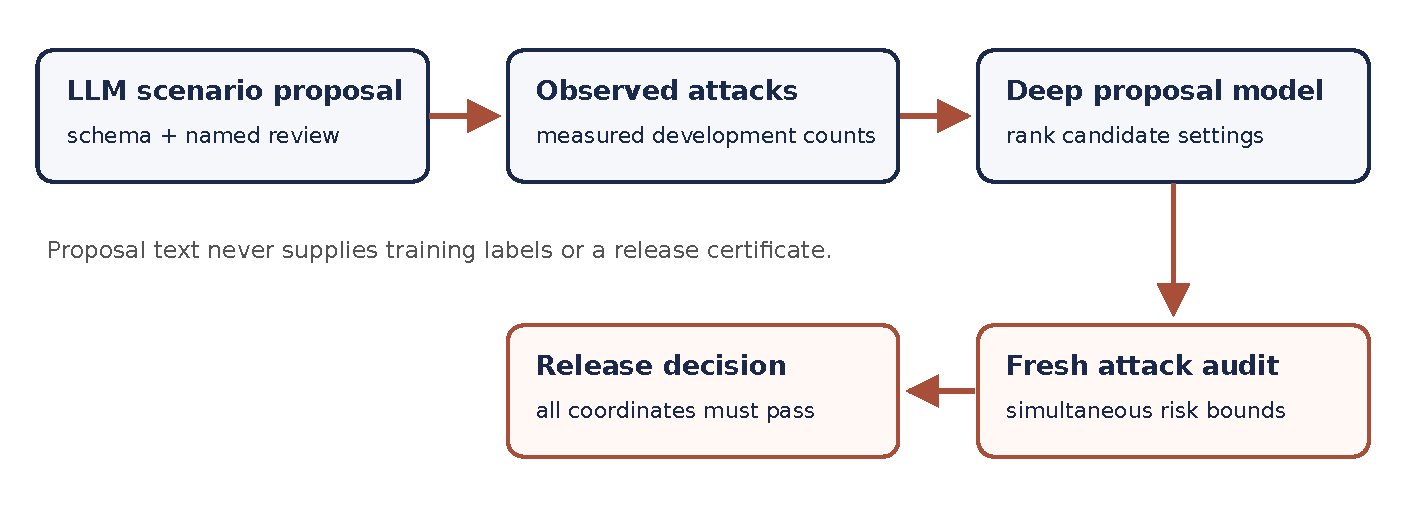
\includegraphics[width=.9\linewidth]{../diagrams/sentry_r_loop.pdf}
\caption{The three evidence streams of SENTRY-R. Proposals change the development programme; only fresh audit outcomes enter the gate.}\label{fig:sentry}
\end{figure}

\subsection{Network and training objective}
Let $x_r\in\mathbb R^d$ hold the features of development row $r=1,\ldots,N$ (mechanism, sampling, auxiliary information and attacker), standardised as $(x_{rk}-m_k)/\zeta_k$ with means $m_k$ and scales $\zeta_k$ estimated on training programmes only. Output $j=1,\ldots,J$ corresponds to one declared coordinate type. For hidden widths $h_1,\ldots,h_L$ and $\rho(u)=\max(0,u)$,
\begin{equation}\label{eq:net}
H^0=X,\quad Z^\ell=H^{\ell-1}W_\ell+\mathbf 1b_\ell^\top,\quad H^\ell=\rho(Z^\ell),\quad P=\mathrm{sigmoid}(H^LW_{L+1}+\mathbf 1b_{L+1}^\top),
\end{equation}
with $W_1\in\mathbb R^{d\times h_1}$ and $W_{L+1}\in\mathbb R^{h_L\times J}$; $L=0$ gives logistic regression. The \texttt{neural\_trust} module fixes $L=1$; the \texttt{sentry\_r} module makes $L$ configurable. If $K_{rj}$ of $B_{rj}$ prechosen development attacks succeed, the counted Bernoulli objective is
\begin{equation}\label{eq:loss}
\mathcal L(\phi)=-\frac1{B_\bullet}\sum_{r,j}\bigl[K_{rj}\log P_{rj}+(B_{rj}-K_{rj})\log(1-P_{rj})\bigr]+\frac\lambda2\sum_{\ell=1}^{L+1}\|W_\ell\|_F^2,\qquad B_\bullet=\sum_{r,j}B_{rj}.
\end{equation}
If $K_{rj}\sim\mathrm{Binom}(B_{rj},\pi_j(x_r))$ given fixed features and trial counts, the expected excess unregularised loss at prediction $p$ is $(B_{rj}/B_\bullet)D_{\rm KL}(\mathrm{Bern}(\pi_j(x_r))\,\|\,\mathrm{Bern}(p))$. This identity names the target of training; it does not show that a fitted model is calibrated or that it transfers to a new programme.

\subsection{Gradients and size}
With output error $G^{L+1}=(B\odot P-K)/B_\bullet$, backpropagation \cite{rumelhart1986} gives
\begin{align}\label{eq:gradient}
G^\ell&=(G^{\ell+1}W_{\ell+1}^\top)\odot\mathbf 1_{Z^\ell>0},\qquad\ell=L,\ldots,1,\\
\nabla_{W_\ell}\mathcal L&=(H^{\ell-1})^\top G^\ell+\lambda W_\ell,\qquad\nabla_{b_\ell}\mathcal L=\mathbf 1^\top G^\ell,\qquad\ell=1,\ldots,L+1,\nonumber
\end{align}
with subgradient zero at a zero preactivation. For common width $h$ the parameter count and cost per example are $O(dh+(L-1)h^2+hJ)$. The number of audit trials needed to certify a small tolerance is set by Proposition~\ref{M-prop:cost}, whatever the width or depth.

\subsection{How predictions enter the audit}
A fixed prediction $\widehat r_i$ can serve as the bet $q_{i,b}=\min(\widehat r_i,\tau_i-\eta)$ for a declared $\eta>0$, provided it was computed without seeing $X_{i,b}$. Later bets may use earlier audit outcomes, and the model may be retrained on them for later bets. This is a condition on timing, not on accuracy. Retraining in this way is not allowed for a fixed-sample family, whose planned sizes must not be changed after final outcomes are seen.

\subsection{Shift and sensitivity}
Calibration on development programmes does not identify the risk of an untested attacker. If a total variation distance between the declared attack law $P$ and a future law $Q$ is justified to be at most $\Delta_{\rm TV}$, then $|r_P-r_Q|\le\Delta_{\rm TV}$ for a binary success event; a change in a network embedding is not an estimate of $\Delta_{\rm TV}$. Because the sigmoid has slope at most $1/4$ and ReLU is 1-Lipschitz, at fixed weights and in raw feature units
\begin{equation}\label{eq:lipschitz}
\|\widehat{\boldsymbol r}(x)-\widehat{\boldsymbol r}(x')\|_2\le\frac14\Bigl(\prod_{\ell=1}^{L+1}\|W_\ell\|_2\Bigr)\max_k\zeta_k^{-1}\,\|x-x'\|_2 .
\end{equation}
This bounds the sensitivity of the network's outputs, not disclosure risk.

\subsection{Benchmark}
On a synthetic programme law with 320 training rows, 100 rows for early stopping and a separate test set of 2,000 rows, both models were trained to convergence (width 24, patience 150, at most 6,000 epochs) over 10 seeds. Mean test log loss was 0.2556 (SD 0.0043) for logistic regression and 0.2576 (SD 0.0047) for a three-layer ReLU network; Brier scores \cite{brier1950} were 0.0727 (SD 0.0017) and 0.0735 (SD 0.0018). Logistic regression had the lower log loss in all 10 seeds, by 0.0020 on average. The rows do not come from the credit register or the public files. The table shows that the pipeline runs, not that depth helps.

\subsection{What the software enforces}
The SENTRY-R code freezes $\alpha$, the planned trial counts, an owner, an expiry date and the identifiers of development evidence before the final audit. The audit refuses changed trial counts and reused development evidence and, with the command-line ledger, a second audit of one frozen record. The code records, but does not enforce, the order of LLM proposals, development attacks and final audits. The quantity $1-U_j/\tau_j$ reported beside a candidate is its audited margin; the network does not produce it.
